\documentclass[twocolumn]{phdsymp} %!PN
\usepackage[english]{babel}
\usepackage{tikz}						%Toevoegen van tikz figuren
\usepackage{pgfplots}					%Grafieken plotten in tikz figuren
\usepackage{graphicx}                   % Om figuren te kunnen verwerken
\usepackage{graphics}					% Om figuren te verwerken.

\graphicspath{{../boek/figuren/}}               % De plaats waar latex zijn figuren gaat halen.

%Do not split footnotes
\interfootnotelinepenalty=10000

\usepackage{times}

\hyphenation{}

\def\BibTeX{{\rm B\kern-.05em{\sc i\kern-.025em b}\kern-.08em
    T\kern-.1667em\lower.7ex\hbox{E}\kern-.125emX}}

\newtheorem{theorem}{Theorem}

\begin{document}

\title{Real-time signal synchronization with acoustic fingerprinting} %!PN

\author{Ward Van Assche}

\supervisor{Joren Six, Marleen Denert}

\maketitle

\begin{abstract}
Many experiments use sensors such as accelerometers and pressure sensors. A common problem after these experiments is the synchronization of data of each sensor. The current synchronization system requires each sensor to be connected to a microphone recording the sound of the environment. With efficient audio-to-audio alignment techniques the latency can be detected very accurately. Because the detection is a post-processing step a real-time and more user-friendly solution is desirable. This paper explores the possibilities to do this. To use the current synchronization algorithms in real-time they had to be changed and optimized in different ways. The new system resulted in a Max/MSP module which makes it possible to run the synchronization in real-time without writing a single line of code.
\end{abstract}

\begin{keywords}
Signal Synchronization, Audio Alignment, Real-Time, Acoustic Fingerprinting, Cross-covariance, Digital Signal Processing
\end{keywords}

\section{Introduction}


\PARstart{E}{xperiments} in various research areas use sensors and video cameras to capture the environment.  Before sensor data and video recordings can be analyzed properly they have to be synchronized accurately in time. This is rather difficult because of various reasons. The first problem is that the sensor datastreams can be heterogeneous: the sample rate can vary and the resulted data can be different (video data or numerical samples). Another difficulty is to cope with the fact that some data sources are sampled unreliably. This can lead to dropped samples and drift which cause unexpected latency changes. 

Most techniques require a post-processing step: the data has to be synchronized manually or by software \emph{after} the experiment. This is impractical and time-consuming. A technique which can avoid this is desirable.

The most straightforward way to perform synchronization is by adding markers. This technique is described in \cite{bannach2009automatic}. How a marker is placed depends on the type of stream. A short sound can add a marker in an audio stream, a bright flash can do this in a video stream. The latency can be found by calculating the difference between marker positions. The usability of this method is limited because of its poor scalability. The synchronization of a large number of streams can be very challenging. Dropped samples and drift can only be detected when the markers are repeated each time interval, which is impractical. Actual synchronization using this technique is only possible as a post-processing operation.

In \cite{jaimovich2010synchronization} a method is described which uses a clock signal to synchronize streams in real-time. However this method avoids the post-processing step it does not fit the requirements: each device (sensor, video camera) should accept a clock-signal as input. Because these devices (especially cameras) are very expensive this method is not feasible for the stated problem.

In \cite{six2015multimodal} the stated problem is approached in an entirely different way. The described method does not try to synchronize the streams directly. Instead, the (recorded) environment sound is embedded in each stream. This ploy reduces the initial problem to audio-to-audio alignment. Because the recorded environment sound is almost the same for each stream, the problem is much easier to tackle. The audio-to-audio algorithms described in the article perform very well. The latency can be detected with a precision less than 1ms. However the article only describes a post-processing approach, the used algorithms look very interesting.

The next part of this paper will describe a method to synchronize streams in real-time using the algorithms mentioned in the previous article. The word ``real-time'' can be ambiguous in a signal-processing context. Therefore it's important to specify some requirements for a real-time system. Because the latency-detecting algorithms need some amount of audio in order to determine the latency it's impossible to immediately output the synchronized signals. In this paper the real-time restriction refers to the fact that the synchronization algorithms are executed while the sensors are collecting data. The post-processing step should be avoided.

\section{Determining latency}

The method described in \cite{six2015multimodal} uses two latency detecting algorithms which are complementary. By combining them, latency can be detected accurately.

\subsection{Acoustic fingerprinting}
Acoustic fingerprinting is a fast and robust technique for comparing audio fragments. A method using acoustic fingerprinting is described in \cite{Wang2003a}. The method uses fingerprints based on spectral peaks. Each fingerprint contains condensed information based on typical audio properties. This technique allows finding similar audio fragments ignoring noise and other disturbing background sounds. 

However the initial application was identifying an audio recording using a huge database containing a myriad of fingerprints, it's also possible to compare the fingerprints of recordings mutually. The latency can be detected by calculating the offset between the fingerprints. The precision varies around $16ms$ to $32ms$ depending on the used parameters.

\subsection{Cross-covariance}
The cross-covariance (also referred to as cross-correlation) is a calculation which measures the degree of similarity between two time sequences. Because an audio signal is a time sequence, this calculation can be used for determining the latency. When the cross-covariance value is calculated for each possible shift between two audio fragments, the shift with the highest result determines the latency.

This method can determine the latency to the nearest sample. The precision in milliseconds depends on the sample rate: when the sample rate is $8000Hz$ the maximum precision is $ 1/8000 Hz = 0.125ms $.

A disadvantage of this method is its performance. The time complexity of the algorithm is $ O(n^2) $ where $ n $ is the number of samples in each signal. Finding the latency between two audio fragments of $10s$ at a sample rate of $8000Hz$ would asymptotically result in $ 6.4 \cdot 10^9 $ computations, which is impracticable on a regular computer.

\subsection{Refining the results}

The two previously described algorithms are very complementary. Acoustic fingerprinting allows finding the latency very fast and robustly. The cross-covariance algorithm can detect the latency between two tiny pieces of audio very accurately. These advantages can be easily combined.

By determining the raw latency with acoustic fingerprinting, the number of samples used in the cross-covariance calculation can be limited. By cutting the raw latency from the corresponding audio fragment, the new latency is reduced. When the acoustic fingerprinting algorithm uses a precision of $32ms$, the cross covariance should be calculated on two audio fragments of at least $256$ samples (when the sample rate is $8000Hz$). This asymptotically results in $65\,536$ computations, which is much more feasible than without the acoustic fingerprinting step.

\subsection{Optimizations}

Many optimization are applied to the latency-detecting algorithms. The most important one is the repeated execution of the cross-covariance algorithm. The cross-covariance algorithm is very sensitive to noise and other undesirable sounds. Since the algorithm calculates similarity of waveforms, these sounds can be harmful to the final result.

Because the cross-covariance algorithm is executed on a very tiny piece of audio it can be executed multiple times on a slightly different location. The most frequent latency is the final result of the algorithm. However the results are much more accurate after this optimization, the influence on the performance is limited. This because the time complexity function remains the same.

\section{Buffering streams}

In order to avoid the post-processing step the real-time streams have to be buffered.
The algorithms are executed on the consecutive buffers of each stream. The buffer size ($t$) will be expressed in seconds of audio it can contain. It determines the maximum latency which can be detected. A minimum length of $10s$ is desirable to make the algorithms perform well. In order to detect latency changes as fast as possible, a step size ($s$) has to be chosen (also expressed in seconds). The step size determines the interval between the moments a new buffer for each stream is created. When the step size is smaller than the buffer size, the overlap between two consecutive buffers is equal to $ t - s $.

\begin{figure}[ht]
	\begin{center}
		\begin{tikzpicture}[scale=0.9]
\begin{axis}[
xlabel={Tijd (seconden)},
xmin=170,xmax=200,
ymin=0,ymax=1,
legend style={
	cells={anchor=west},
	legend pos=outer north east,
},
yticklabels={,,},
xticklabel style={grid=major},
extra x ticks={176,177,186,187},
extra x tick labels={,,,},
extra tick style={grid=major, grid style={dotted}},
hide y axis
]
\addplot[thick,black] graphics[xmin=140,ymin=0,xmax=200,ymax=1] {wave.png};

after end axis/.code={
	\draw[black,<->] (axis cs:175,0.1) -- (axis cs:185,0.1)	node [pos=0.5,above,font=\scriptsize] {buffer $i-1$};
	
	\draw[black,<->] (axis cs:176,0.2) -- (axis cs:186,0.2)	node [pos=0.5,above,font=\scriptsize] {buffer $i$};
	
	\draw[black,<->] (axis cs:177,0.3) -- (axis cs:187,0.3)	node [pos=0.5,above,font=\scriptsize] {buffer $i+1$};
}]

%\node at (50,18) [] {\small$\Delta t$};
%\addplot[style=dotted,color=gray,very thick] coordinates{ (90,129)
%	(90,100)}; 
%\addplot[style=dotted,color=gray,very thick] coordinates{
%	(150,190) (150,100)};
%\addplot[color=black,<->,thick] coordinates{ (90,115)
%	(150,115)};

\end{axis}

\end{tikzpicture}
		\caption{\label{buffers}Visualization of a buffer containing $10s$ of audio with a step size of $5s$.}
	\end{center}
\end{figure}

Both the buffer size and step size influence the time between a latency change and its detection. Since the latency can only be detected when more than half of the buffer contains the modified latency, the best case detection speed is equal to $ t/2 $. By applying a smaller step size the worst case scenario can be improved: it is equal to $ t/2 + s $. Figure \ref{buffers} shows a buffer where $t=10$ and $s=5$.

\newcommand{\datafiltergraph}[1]
{
	\begin{tikzpicture}[scale=0.9]
		\begin{axis}[
		ylabel={Latency (ms)},
		xtick ={0,5,10,15,...,35},
		ytick ={60,80,...,180},
		ymin = 60,
		ymax = 180,
		height = 5cm,
		width = 8cm
		]
		\addplot [mark=none] table {#1.dat};
		\end{axis}
	\end{tikzpicture}
}

\section{Latency filters}
The avoidance of the post-processing step makes it harder to manually fix potential errors. When using audio recordings of poor quality, it's recommended to use a moving median latency filter. By using this filter the consecutive latencies are pushed in a queue. Each time a new latency is determined, the median of the values in the queue is returned. Depending on the queue size, some peaks in the consecutive latencies are flattened. 

\begin{figure}[th!]
	\begin{center}
		\datafiltergraph{../boek/latencydata}
		\caption{\label{latency_nofilter}The sequence of latencies without filtering.}
	\end{center}
\end{figure}

\begin{figure}[th!]
	\begin{center}
		\datafiltergraph{../boek/median5data}
		\caption{\label{latency_filter}The sequence of latencies after filtering.}
	\end{center}
\end{figure}

Figure \ref{latency_nofilter} shows a sequence of latencies without filtering, figure \ref{latency_filter} shows the same sequence after filtering with a moving-median 
 
\section{Synchronization}
The actual synchronization is performed by adding silence to each stream. The latencies of each stream are converted to the amount of silence which has to be added to each stream. It's a good practice to synchronize the streams by adding whitespace. However this can also be done by dropping samples, the extra loss of data is undesirable.

\section{Results}
This research resulted in two Max/MSP modules\footnote{Max/MSP is software and a visual programming language which allows processing audio and video signals. This can be done by connecting existing modules each having a specific task. Max/MSP allows writing own modules in Java or C++.}. One module is able to read sensor datastreams accompanied by an audiostream from a \emph{Teensy microcontroller} into the Max/MSP environment. The second module is designed to perform the actual synchronization.

\subsection{Using a Teensy}

A Teensy is a microcontroller which can be used to attach several sensors to a microphone with a negligible latency between the streams. This property is very useful for the stated problem. Because the actual synchronization is performed in Max/MSP it's required to read the analog Teensy pins into Max/MSP which isn't natively supported. To support this, a new module had to be written: the \mbox{\emph{TeensyReader}}.
\begin{figure}[ht]
	\begin{center}
		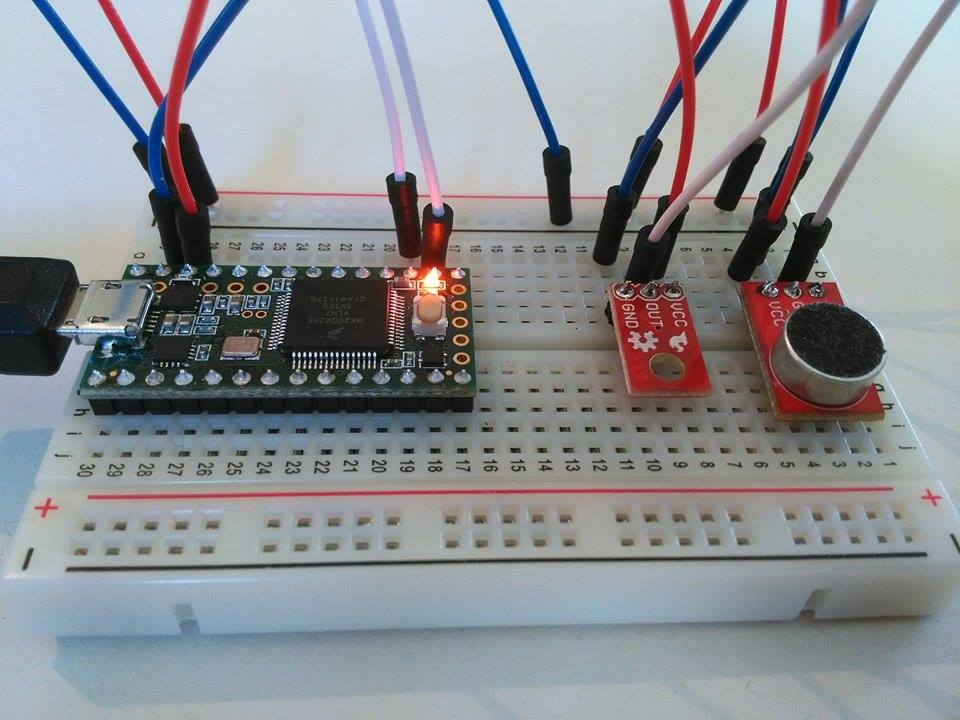
\includegraphics[width=0.3\textwidth]{../boek/figuren/teensy.jpg}
		\caption{\label{teensy}A Teensy microcontroller.}
	\end{center}
\end{figure}
The module requires several parameters: port name, sample rate of the Teensy, index of the first analog pin (A3 $\rightarrow$ 3), index of the audio pin (starting at 0 for the first analog pin) and the number of analog pins to read.

Figure \ref{teensy} shows a picture of a Teensy connected to a microphone and an infrared sensor.

\begin{figure}[ht]
	\begin{center}
		\includegraphics[width=0.3\textwidth]{../boek/figuren/teensyreader.png}
		\caption{\label{teensyreader}The TeensyReader module in Max/MSP.}
	\end{center}
\end{figure}

Figure \ref{teensyreader} shows the TeensyReader module reading signals from the infrared sensor and microphone. The signals are displayed on two scopes.


\subsection{The Sync module}

The \emph{Sync} module performs the actual synchronization. It uses the software library which is responsible for buffering the streams and calculating the latency. The module uses the latency to add silence to each stream and output the synchronized streams.

The module requires one parameter which is a character representation of the stream structure. The parameter is a comma separated string where each part consists of one '\texttt{a}' character and any number of '\texttt{d}' characters. An audio stream which should be used for synchronization (using the audio-to-audio alignment algorithms) is represented by '\texttt{a}', an attached data stream by '\texttt{d}'. The character order determines the order of inlets and outlets of the module.

Figure \ref{sync} shows the Sync module created with parameter \texttt{dad,addd}. The synchronized outlets are sent to the \emph{sfrecord} module which writes the synchronized streams to a file.

\begin{figure}[ht]
	\begin{center}
		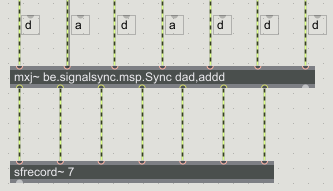
\includegraphics[width=0.4\textwidth]{../boek/figuren/syncwrite.png}
		\caption{\label{sync}The Sync module in Max/MSP. The data patch cable is labeled with \texttt{d}, an audio patch cable with \texttt{a}.}
	\end{center}
\end{figure}

\section{Conclusion}
Several tests proved that the synchronization works very well without the post-processing step. Even audio recorded from poor quality can be synchronized easily avoiding the post-processing step. 

\bibliographystyle{phdsymp}
\bibliography{../bronnen/bronnen}

\end{document}
